\documentclass[12pt]{article}

\usepackage{graphicx}
\usepackage{tabularx}
\usepackage{lastpage}
\usepackage{tikz}
\usetikzlibrary{automata}
\usepackage{qtree}
\usepackage{enumitem}
\usepackage{amsmath}

\date{\today}
\author{Robert Krency \\ Cody Long \\ Noelle Nieves}
\title{Assignment 1}

% Geometry 
\usepackage[margin=1in]{geometry}

% Fancy Header
\usepackage{fancyhdr}
\fancyhf{}
\lhead{CSC 460}
\rhead{Krency - Long - Nieves}
\cfoot{Page \thepage \hspace{1pt} of \pageref{LastPage}}

% Add vertical spacing to tables
\renewcommand{\arraystretch}{1.4}

% Document
\begin{document}

\maketitle
\thispagestyle{fancy}

\section*{Q3}

\begin{enumerate}[label=(\alph*)]
    \item $(ab^*a)|(ba^*b)$
    \item $a(b?cda)*$
    \item $(ab^*c)?$
\end{enumerate}

\section*{Q4}

\subsection*{(a) $(a\ |\ (bc)^*\ d)^+$}

\begin{center}
    
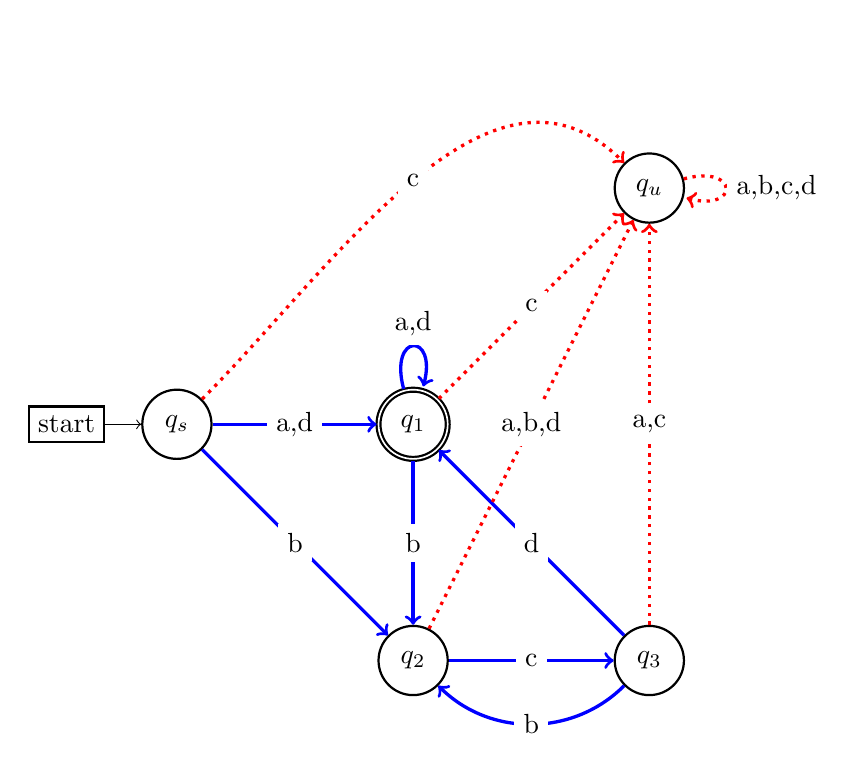
\begin{tikzpicture}

    \begin{scope}[every node/.style={circle,thick,draw}]
        \node[initial,state] (1) at (0,0) {$q_s$};
        \node[state,accepting] (2) at (3,0) {$q_1$};
        \node[state] (3) at (6,-3) {$q_3$};
        \node[state] (4) at (3,-3) {$q_2$};
        \node[state] (5) at (6,3) {$q_u$}; % Unaccepted Node %
    \end{scope}

    \begin{scope}[every node/.style={fill=white,rectangle}, every edge/.style={draw=blue,very thick}]
        \path [->] (1) edge node {a,d} (2);
        \path [->] (2) edge [loop above] node {a,d} (2);
        \path [->] (1) edge node {b} (4);
        \path [->] (2) edge node {b} (4);
        \path [->] (4) edge node {c} (3);
        \path [->] (3) edge node {d} (2);
        \path [->] (3) edge [out=225,in=315] node {b} (4);
    \end{scope}

    \begin{scope}[every node/.style={fill=white,rectangle}, every edge/.style={draw=red,very thick,dotted}]
        \path [->] (1) edge [out=45, in=135] node {c} (5);
        \path [->] (2) edge node {c} (5);
        \path [->] (4) edge node {a,b,d} (5);
        \path [->] (3) edge node {a,c} (5);
        \path [->] (5) edge [loop right] node {a,b,c,d} (5);
    \end{scope}

\end{tikzpicture}
\end{center}

\pagebreak
\subsection*{(b) $(((0|1)^*(2|3)^+)|0011)$}

\begin{center}
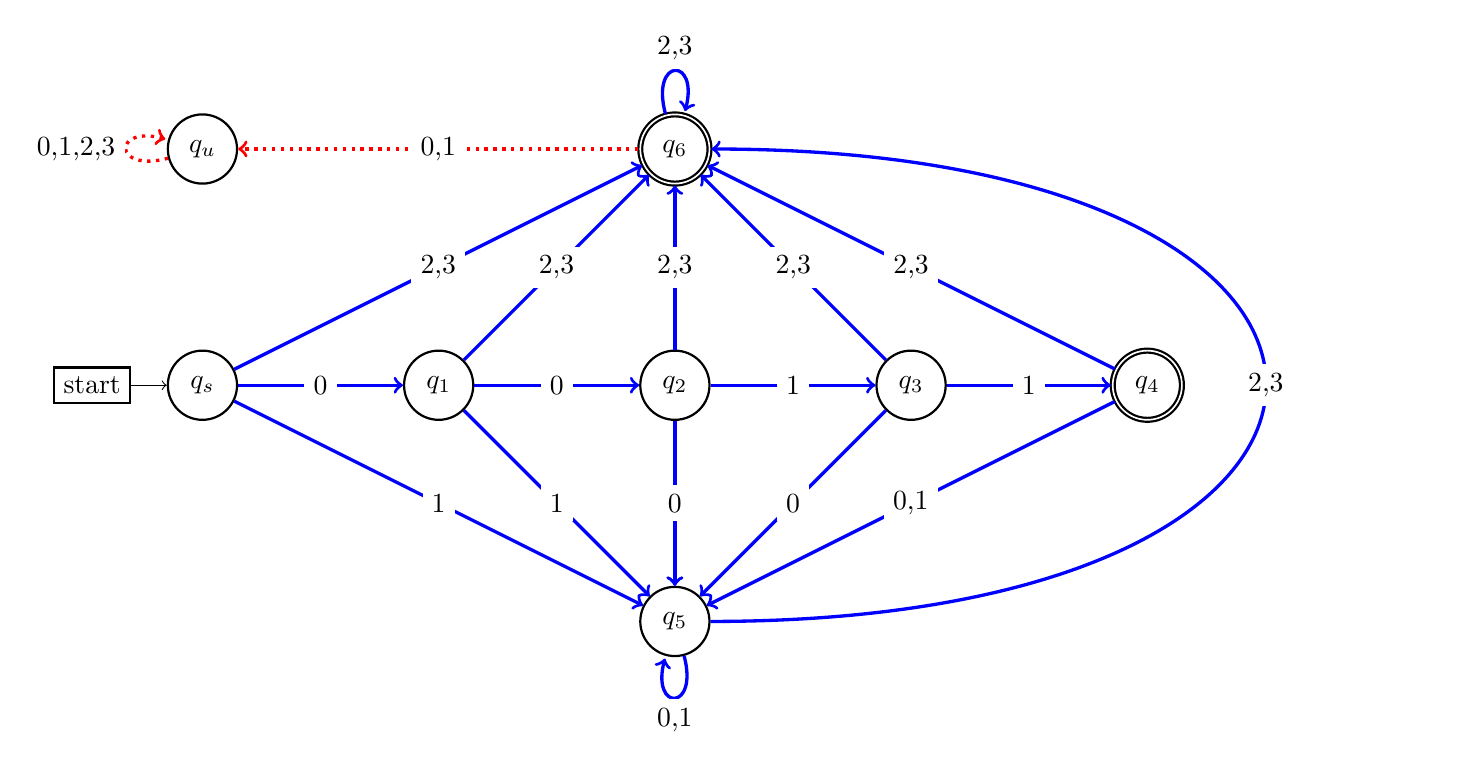
\begin{tikzpicture}

    \begin{scope}[every node/.style={circle,thick,draw}]
        \node[initial,state] (1) at (0,0) {$q_s$};
        \node[state] (2) at (3,0) {$q_1$};
        \node[state] (3) at (6,0) {$q_2$};
        \node[state] (4) at (9,0) {$q_3$};
        \node[state,accepting] (5) at (12,0) {$q_4$};
        \node[state] (6) at (6,-3) {$q_5$};
        \node[state,accepting] (7) at (6,3) {$q_6$};
        \node[state] (8) at (0,3) {$q_u$}; % Unaccepted Node %
    \end{scope}

    \begin{scope}[every node/.style={fill=white,rectangle}, every edge/.style={draw=blue,very thick}]
        % Path for 0011 %
        \path [->] (1) edge node {0} (2);
        \path [->] (2) edge node {0} (3);
        \path [->] (3) edge node {1} (4);
        \path [->] (4) edge node {1} (5);

        % Other path %
        \path [->] (7) edge [loop above] node {2,3} (7);
        \path [->] (6) edge [loop below] node {0,1} (6);
        \path [->] (1) edge node {1} (6);
        \path [->] (2) edge node {1} (6);
        \path [->] (3) edge node {0} (6);
        \path [->] (3) edge node {0} (6);
        \path [->] (4) edge node {0} (6);
        \path [->] (5) edge node {0,1} (6);
        \path [->] (1) edge node {2,3} (7);
        \path [->] (2) edge node {2,3} (7);
        \path [->] (3) edge node {2,3} (7);
        \path [->] (4) edge node {2,3} (7);
        \path [->] (5) edge node {2,3} (7);
        \path [->] (6) edge [out=0, in=0, looseness=4] node {2,3} (7);

    \end{scope}

    \begin{scope}[every node/.style={fill=white,rectangle}, every edge/.style={draw=red,very thick,dotted}]
        \path [->] (7) edge node {0,1} (8);
        \path [->] (8) edge [loop left] node {0,1,2,3} (8);
    \end{scope}

\end{tikzpicture}

\end{center}

\subsection*{(c) $(a $Not$(a))^*aaa$}

\begin{center}
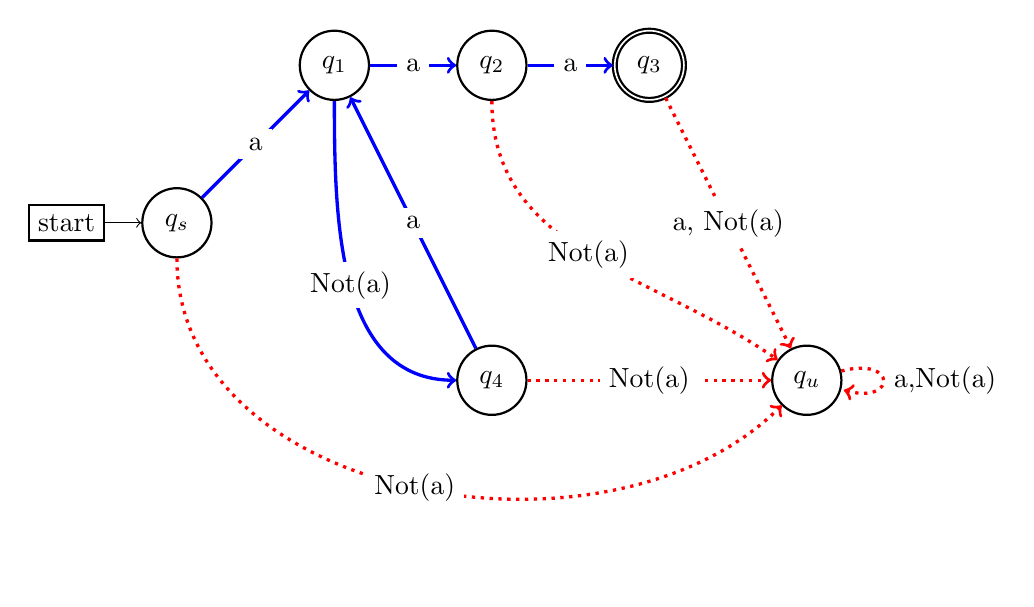
\begin{tikzpicture}

    \begin{scope}[every node/.style={circle,thick,draw}]
        \node[initial,state] (1) at (0,0) {$q_s$}; % Start node
        \node[state] (2) at (8,-2) {$q_u$}; % Unaccepted Node %
        \node[state] (3) at (2,2) {$q_1$};
        \node[state] (4) at (4,2) {$q_2$};
        \node[state,accepting] (5) at (6,2) {$q_3$};
        \node[state] (6) at (4,-2) {$q_4$};
    \end{scope}

    \begin{scope}[every node/.style={fill=white,rectangle}, every edge/.style={draw=blue,very thick}]
        % Path for 0011 %
        \path [->] (1) edge node {a} (3);
        \path [->] (3) edge node {a} (4);
        \path [->] (4) edge node {a} (5);
        \path [->] (6) edge node {a} (3);
        \path [->] (3) edge [out=270, in=180] node {Not(a)} (6);

    \end{scope}

    \begin{scope}[every node/.style={fill=white,rectangle}, every edge/.style={draw=red,very thick,dotted}]
        \path [->] (5) edge node {a, Not(a)} (2);
        \path [->] (1) edge [out=270,in=225,looseness=1] node {Not(a)} (2);
        \path [->] (4) edge [out=270,in=145,looseness=1] node {Not(a)} (2);
        \path [->] (6) edge node {Not(a)} (2);
        \path [->] (2) edge [loop right] node {a,Not(a)} (2);
    \end{scope}

\end{tikzpicture}
\end{center}

\section*{Q5}

$\bigl( [1-9][0-9]^*\ |\ 0 \bigr) \ .\ \bigl( [0-9]^*[1-9]\ |\ 0 \bigr) $


\end{document}